\begin{boxC}
    ما برای الگوریتم 
    \lr{Expect Maximization}
    روابط زیر را در اختیار داریم :
    
    \begin{equation*}
        P(d) = P(\Theta_{1}) P(d | \Theta_{1}) + P(\Theta_{2}) P(d | \Theta_{2}) 
    \end{equation*}

    \begin{equation*}
        P(d | \Lambda) = \sum_{i = 1}^{k} (P(\Theta_{i}) \prod_{w \in V} P(w | \Theta_{i}) ^ {c(w , d)}) 
    \end{equation*}

    \begin{equation*}
        \Lambda ^ * = argmax_{\Lambda} P(d | \Lambda)
    \end{equation*}
    
\end{boxC}


\begin{boxK}
هموارسازی لاپلاسی الگوریتمی برای هموار کردن یک شبکه چند ضلعی است. برای هر راس در یک مش، یک موقعیت جدید بر اساس اطلاعات محلی (مانند موقعیت همسایگان) انتخاب می شود و راس به آنجا منتقل می شود.
در صورتی که یک مش از نظر توپولوژیکی یک شبکه مستطیل شکل باشد
(یعنی هر رأس داخلی به چهار همسایه متصل است)
سپس این عملیات لاپلاسی مش را تولید می کند.

میزان احتمال وجود یک ترم خاص در یک 
\lr{Cluster}
به صورت هموارساز لاپلاس محاسبه شده‌است.

با توجه به این که در هر 
\lr{Cluster}
ما ۳ ترم منحصربفرد داریم ، تعداد گره‌های ما ۳ تا خواهد بود.

به ازای هموارساز با فاکتور ۱ خواهیم داشت :

\begin{equation*}
    P(A | Cluster1) = \frac{4 + 1}{9 + 3}    
\end{equation*}
\end{boxK}

\begin{figure}[h]
    \centering
    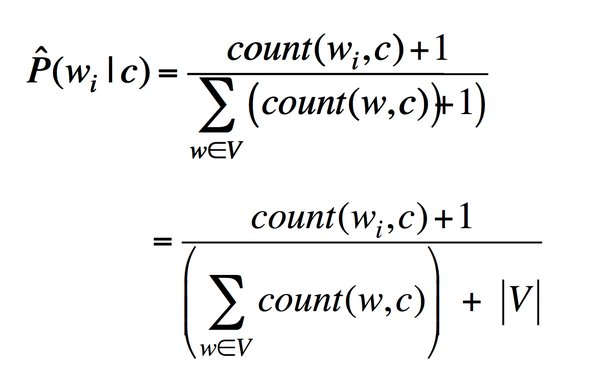
\includegraphics
    [width = 0.4\textwidth]
    {IR5/image/laplacian_smoothing.jpeg}
    \caption{رابطه هموارساز لاپلاسی برای جلوگیری از وجود احتمال صفر برای یک کلمه}
    \label{fig:enter-label}
\end{figure}


\begin{boxD}
    \begin{equation*}
        P(\Theta_{1}) = \frac{3}{4}
    \end{equation*}

    \begin{equation*}
        P(\Theta_{2}) = \frac{1}{4}
    \end{equation*}

    \begin{equation*}
        P(A | Cluster1) = \frac{5}{12}
    \end{equation*}

    \begin{equation*}
        P(B | Cluster1) = \frac{3}{12}
    \end{equation*}

    \begin{equation*}
        P(C | Cluster1) = \frac{1}{12}
    \end{equation*}

    \begin{equation*}
        P(D | Cluster1) = \frac{4}{12}
    \end{equation*}

    -------------------------------------------------------

    \begin{equation*}
        P(A | Cluster2) = \frac{2}{8}
    \end{equation*}

    \begin{equation*}
        P(B | Cluster2) = \frac{3}{8}
    \end{equation*}

    \begin{equation*}
        P(C | Cluster2) = \frac{3}{8}
    \end{equation*}

    \begin{equation*}
        P(D | Cluster2) = \frac{1}{8}
    \end{equation*}

    
\end{boxD}



\begin{boxD}
\begin{equation*}
    P(Document1 | Cluster1) = \frac{3}{4} * (\frac{5}{12}) ^ 2 * \frac{3}{12} = 0.032552083 (X1)
\end{equation*}

\begin{equation*}
    P(Document1 | Cluster2) = \frac{1}{4} * (\frac{2}{8}) ^ 2 * \frac{3}{8} = 0.005859375 (Y1)
\end{equation*}

\begin{center}
    \color{red}
    \lr{Document1 Assigned to Cluster1}
\end{center}

-------------------------------------------------------

\begin{equation*}
    P(Document2 | Cluster1) = \frac{3}{4} * (\frac{3}{12}) ^ 2 * (\frac{1}{12}) ^ 2 * \frac{5}{12} = 0.000135634 (X2)
\end{equation*}

\begin{equation*}
    P(Document2 | Cluster2) = \frac{1}{4} * (\frac{3}{8}) ^ 2 * (\frac{3}{8}) ^ 2 * \frac{2}{8} = 0.001235962 (Y2)
\end{equation*}

\begin{center}
    \color{red}
    \lr{Document2 Assigned to Cluster2}
\end{center}

-------------------------------------------------------

\begin{equation*}
    P(Document3 | Cluster1) = \frac{3}{4} * \frac{3}{12}  * \frac{5}{12} * (\frac{4}{12}) ^ 2 = 0.008680556 (X3)
\end{equation*}

\begin{equation*}
    P(Document3 | Cluster2) = \frac{1}{4} * \frac{3}{8}  * \frac{2}{8} * (\frac{1}{8}) ^ 2 = 0.000366211 (Y3)
\end{equation*}

\begin{center}
    \color{red}
    \lr{Document3 Assigned to Cluster1}
\end{center}

-------------------------------------------------------

\begin{equation*}
    P(Document4 | Cluster1) = \frac{3}{4} * \frac{5}{12} * \frac{4}{12} = 0.10416166667 (X4)
\end{equation*}

\begin{equation*}
    P(Document4 | Cluster2) = \frac{1}{4} * \frac{2}{8} * \frac{1}{8} = 0.0078125 (Y4)
\end{equation*}

\begin{center}
    \color{red}
    \lr{Document4 Assigned to Cluster1}
\end{center}

\end{boxD}

\begin{boxK}
    مرحله به‌روزرسانی میزان احتمال هریک از خوشه‌ها : 
    
    \begin{equation*}
        P(\Theta_{1}) = \frac{X1 + X2 + X3 + X4}{4} = 0.364
    \end{equation*}

    \begin{equation*}
        P(\Theta_{2}) = \frac{Y1 + Y2 + Y3 + Y4}{4} = 0.003825
    \end{equation*}
\end{boxK}

\begin{boxD}
    \begin{equation*}
        Manhatan-Dist(D1 , C1) = 3
    \end{equation*}

    \begin{equation*}
        Manhatan-Dist(D1 , C2) = 4
    \end{equation*}

    \begin{center}
    \color{red}
    \lr{Document1 Assigned to C1.}    
    \end{center}

-----------------------------------------------------------

    \begin{equation*}
        Manhatan-Dist(D2 , C1) = 5
    \end{equation*}

    \begin{equation*}
        Manhatan-Dist(D2 , C2) = 2
    \end{equation*}

    \begin{center}
    \color{red}
    \lr{Document2 Assigned to C2}
    \end{center}

-----------------------------------------------------------

    \begin{equation*}
        Manhatan-Dist(D3 , C1) = 2
    \end{equation*}

    \begin{equation*}
        Manhatan-Dist(D3 , C2) = 5
    \end{equation*}

    \begin{center}
    \color{red}
    \lr{Document3 Assigned to C1}
    \end{center}
    
-----------------------------------------------------------


    \begin{equation*}
        Manhatan-Dist(D4 , C1) = 0
    \end{equation*}

    \begin{equation*}
        Manhatan-Dist(D4 , C2) = 5
    \end{equation*}

    \begin{center}
        \color{red}
        \lr{Document4 Assigned to C1}
    \end{center}
    
\end{boxD}

\begin{boxK}
    \begin{center}
    \lr{K-Means Clustering}    
    \end{center}

    \begin{equation*}
        Document5 = C A A
    \end{equation*}

    \begin{equation*}
        Manhatan-Dist(D5 , C1) = 3
    \end{equation*}

     \begin{equation*}
        Manhatan-Dist(D5 , C2) = 4
    \end{equation*}

    \begin{center}
    \color{red}
    \lr{Document5 Assigned to C1}
    \end{center}
    % -------------------------------------------------------------------------------



\end{boxK}

\begin{boxK}
    \begin{center}
    \lr{EM generative Model}    
    \end{center}

    \begin{equation*}
        Document5 = C A A
    \end{equation*}

    \begin{equation*}
        P(Document5 | Cluster1) = P(\Theta_{1}) * P(C | Cluster1) * P(A | Cluster1) ^ 2 = 0.005266204
    \end{equation*}

    \begin{equation*}
        P(Document5 | Cluster2) = P(\Theta_{2}) * P(C | Cluster2) * P(A | Cluster2) ^ 2 = 0.000008965
    \end{equation*}

    \begin{center}
    \color{red}
    \lr{Document5 Assigned to C1}
    \end{center}
\end{boxK}

\begin{boxM}
    هر دو رویکرد الگوریتمی داکیومنت ۵ را به کلاستر اول نظیر خواهد کرد.
\end{boxM}


\begin{boxM}
        \lr{EM-Generative}
        و
        \lr{K-Means}
        هر دو الگوریتم‌های خوشه‌بندی هستند که از آن‌ها استفاده زیادی می‌شود.

        مزایای 
        \lr{EM-Generative} : 

        \begin{enumerate}
            \item 
            می‌تواند داده‌های پراکنده و دارای توزیع نامناسب ، مانند مثال همین سوال را تا حد بسیار خوبی بر اساس احتمال 
            \lr{Background}
            مناسب ، خوشه‌بندی کند.

            \item 
            می‌تواند خوشه‌هایی با اشکال ، اندازه‌ها و چگالی متفاوت تولید کند.

            \item 
            \lr{EM-Generative}
            می‌تواند داده‌های از دست رفته را با وارد کردن مقادیر گمشده با استفاده از مدلی که از داده‌های موجود به دست می‌آید، مدیریت کند.

            \item
            \lr{EM-Generative}
            می‌تواند برای شناسایی الگوها در داده‌های با ابعاد بالا با کاهش ابعاد داده‌ها با استفاده از تکنیک‌هایی استفاده شود.
            
            
            
        \end{enumerate}

        معایب 
        \lr{EM-Generative}:
        \begin{enumerate}
            \item 
            تولید 
            \lr{EM}
            می‌تواند از نظر محاسباتی محاسباتی گران باشد ، به خصوص زمانی که با مجموعه داده‌های بزرگ یا ابعاد بالا سروکار داریم.

            \item 
            \lr{EM-Generative}
            نیاز به تنظیم دستی پارامترهای اولیه دارد که اگر دانش قبلی در مورد ساختار داده‌ها وجود نداشته باشد ، می‌تواند چالش‌برانگیز باشد . انتخاب پارامترهای اولیه نیز می‌تواند بر خوشه‌های حاصل تاثیر بگذارد.
            
            \lr{EM}
            ممکن است به یک بهینه محلی همگرا شود یا در یک حالت گیرکند اگر در طول فرآیند تکرار به دقت نظارت و تطبیق داده نشود.

            \item 
            \lr{EM-Generative}
            فرض می‌کند که هر خوشه تابع چگالی خاصی دارد ، که ممکن است همیشه در سناریوهای دنیای واقعی صادق نباشد .

            در چنین مواردی ممکن است نتایج کمتر از حد بهینه ایجاد کند یا به درستی همگرا نشود.
        \end{enumerate}


        مزایای
        \lr{K-Means} :
        \begin{enumerate}
            \item 
            \lr{k-means}
            از نظر محاسباتی کارآمد است و پیاده‌سازی آن آسان است و آن را به یک انتخاب درست برای خوشه‌بندی مجموعه داده‌های بزرگ تبدیل می‌کند.
                     
            \item 
            \lr{K-Means}
            خوشه‌هایی با ابعاد کروی و تقریبا میزان داده برابر تولید می‌کند که در بسیاری از کاربردهایی که این مفروضات درست هستند.
            
            \item
            \lr{K-Means}
            امکان پردازش موازی را فراهم می کند، که می تواند زمان محاسبات را در هنگام برخورد با مجموعه داده های بزرگ یا چندین پردازنده/هسته موجود در یک ماشین/خوشه، به میزان قابل توجهی افزایش دهد.
        \end{enumerate}
        
\end{boxM}

\begin{boxM}
    همانطور که پیش‌تر هم ذکر شد ، رویکرد 
    \lr{EM-Generative}
    برای این توزیع داده بسیار مناسب‌تر خواهد بود . 

    به شرطی که میزان احتمال هر خوشه ، بر اساس دانش قبلی مناسب به وجود بیاید.

    از توزیع هندسی این نقاط ، می‌توان این نتیجه را گرفت که مدل ساده 
    \lr{K-Means}
    قادر به خوشه‌بندی مناسبی برای این داده‌ها نخواهد بود ، چرا که میزان شباهت بین داده‌ها اگر بر اساس فاصله اقلیدسی یا هر نوع فاصله    ، دیگری باشد 
    قادر به ارائه خوشه‌های مناسبی نخواهد بود.

\end{boxM}